\section{Convolutional Networks for Sequence Modelling}

\begin{frame}
	\frametitle{Convolutional Architectures}

	A popular alternative to recurrent architectures is \alert{convolutional} based architectures
	for sequence modelling

	\begin{center}
		\textbf{Example: WaveNet}

		\medskip

		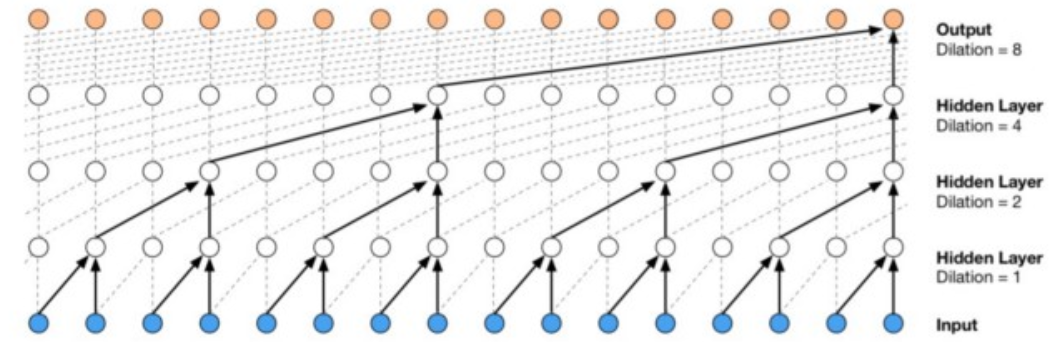
\includegraphics[width=14cm]{figures/wavenet.png}
	\end{center}

	\blfootnote{
		\fullcite{oord2016wave}
	}

\end{frame}

\begin{frame}
	\frametitle{Convolutional vs Recurrent Architectures}

	In practice, there are empirical works demonstrating the superiority of both.

	\medskip

	\begin{center}
		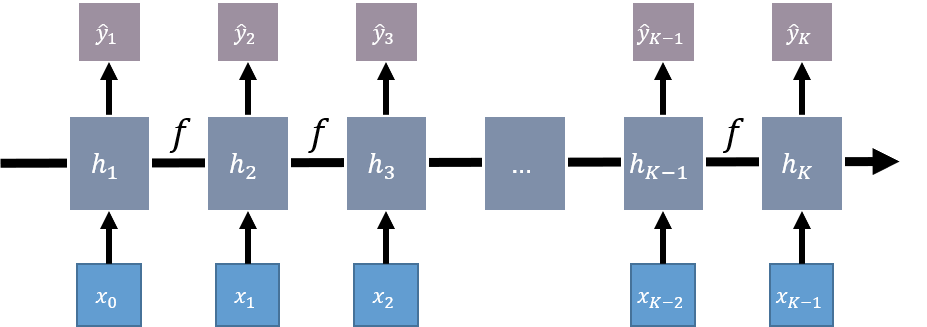
\includegraphics[width=6cm]{figures/recurrent_structure.png}
		\quad
		\textbf{v.s.}
		\quad
		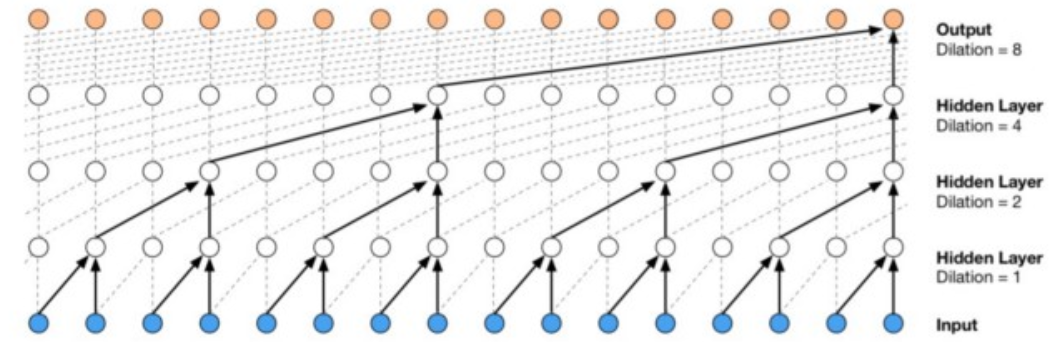
\includegraphics[width=6cm]{figures/wavenet.png}
	\end{center}

    \begin{empheq}[box=\mymath]{gather*}
	\text{
			Is one really better than the other?
	} \\
		\text{
			When should we use convolutional and recurrent architectures?
		}
    \end{empheq}

\end{frame}


\begin{frame}
	\frametitle{The Dilated Convolutional Architecture}

	For discrete sequences, define the dilated convolution operation
	\begin{equation*}
		({\bm{x}} \Conv{}_{\ell} {\bm{w}})(t)
		=
		\sum_{s \in \Z}
		{x}(s)^\tp
		{w}(t- \ell s)
	\end{equation*}

	\pause{}

	The \alert{(dilated) CNN architecture} is
	\begin{equation*}
		\begin{aligned}
			\bm h_{0,i} &= \bm x_i\\
			\bm h_{k+1,i} &= \sigma \left(\sum_{j=1}^{M_k} {\bm w}_{kji} *_{d_k} \bm h_{k,j} \right)\\
			\bm {\hat y} &= \bm h_{K,1}
		\end{aligned}
		\quad
		\begin{tabular}{ll}
			\toprule
			$\bm h_{k,i}$ & hidden state at layer $k$, channel $i$ \\
			$\bm w_{kji}$ & size $\R^l$ convolutional filters \\
			$K$           & \# layers \\
			$M_k$	      & \# channels at layer $k$ \\
			$d_k$ 		  & dilation rate at layer $k$ \\
			\bottomrule
		\end{tabular}
	\end{equation*}
\end{frame}

\begin{frame}
	\frametitle{Linear Convolutional Hypothesis Space}

	As before, turn to linear case $\sigma = \id$ and choose $d_k = l^k$, then
	\begin{equation*}
		\begin{aligned}
			\hcnn^{(l,K,\set{M_k})}
			:=
			\left\{
				\bm x \mapsto \wh{\bm y}
				:
				\bm w_{kji} \in \R^l
			\right\}
		\end{aligned}
		\qquad
		% \begin{aligned}
		\scriptsize
		\begin{cases}
			\bm h_{0,i} = \bm x_i\\
			\bm h_{k+1,i} = \sum_{j=1}^{M_k} {\bm w}_{kji} *_{d_k} \bm h_{k,j} \\
			\bm {\hat y} = \bm h_{K,1}
		\end{cases}
		\normalsize
			% &\bm h_{0,i} = \bm x_i\\
			% &\bm h_{k+1,i} = \sigma \left(\sum_{j=1}^{M_k} {\bm w}_{kji} *_{d_k} \bm h_{k,j} \right)\\
			% &\bm {\hat y} = \bm h_{K,1}
		% \end{aligned}
	\end{equation*}
	with total \# variables $m = l \sum_{k} M_{k}M_{k+1}$

	The full CNN hypothesis space is
	\begin{equation*}
		\hcnn\depen{l} =
		\bigcup_{K \in \mathbb N_+}
		\bigcup_{\set{M_k} \in \mathbb N_+^K}
		\hcnn\depen{l,K,\set{M_k}}.
	\end{equation*}
\end{frame}

\begin{frame}[c]
	\frametitle{Approximation Guarantee (Density)}

	\begin{alertblock}{Theorem [JLL, 2021]}
		Let $\{ \Htar_t : t\in\R \}$ be a family of continuous,
		linear, causal, and time-homogeneous functionals on $\ell^2(\Z,\R^d)$.
		Then, for any $\epsilon > 0$ there exists
		$\wh{\bm H} = \{ \wh{H}_t : t\in \R \} \in \hcnnl$ such that
		\begin{equation*}
			% \sup_{t\in\Z}
			% \| \Htar_t - \wh{H}_t \|
			\| \bm \Htar - \wh{\bm H} \|
			\equiv
			\sup_{t\in\Z}
			\sup_{\| \*x \|_{\ell^2} \leq 1}
			|
			\Htar_t(\*x) - \wh{H}_t(\*x)
			|
			\leq \epsilon.
		\end{equation*}
	\end{alertblock}

	\blfootnote{
		\fullcite{jiang2021approx}
	}

\end{frame}


\begin{frame}
	\frametitle{Principles of CNN Approximation}

	How does CNN approximation work?

	\begin{itemize}[<+->]
		\item Target
		\begin{equation*}
			\Htar_t(\bm x)
			=
			\sum_{s = 0}^{\infty}
			\rho^{(\bm H^*)}(s)^\tp
			x(t-s)
			\qquad
			\text{(Riesz Representation)}
		\end{equation*}
		\item CNN Approximation
		\begin{equation*}
			\begin{aligned}
				\wh{H}_t(\bm x)
				=
				\sum_{s = 0}^{l^K - 1}
				\wh{\rho} (s)^\tp
				x(t-s)
				\qquad
				\wh{\bm \rho}
=
				\sum_{\text{all channels}}
				{\bm w_{K-1}}
				\Conv{}_{l^{K-1}}
				{\bm w_{K-2}}
				\Conv{}_{l^{K-2}}
				\cdots
				\Conv{}_{l^{2}}
				{\bm w_{1}}
				\Conv{}_{l^{1}}
				{\bm w_{0}}
				% \sum_{i_0,1,i_{K-1}}
				% {\bm w}_{K-1,i_{K-1},1}
				% \Conv{}_{l^{K-1}}
				% {\bm w}_{K-2,i_{K-2},i_{K-1}}
				% \Conv{}_{l^{K-2}}
				% \cdots
				% \Conv{}_{l^2}
				% {\bm w}_{1,i_{1},i_{2}}
				% \Conv{}_{l}
				% {\bm w}_{0,i_{0},i_{1}}
			\end{aligned}
		\end{equation*}
		\item
		Error consists of two parts
		\begin{equation*}
			\sup_{\|\bm x\|_{\ell^2} \leq 1}
			| \Htar_t(\bm x) - \wh{H}_t(\bm x) |^2
			\leq
			\underbrace{
				\sum_{s=0}^{l^{K}-1}
				\| \rho^{(\bm H^*)}(s) - \wh{\rho}(s) \|^2
			}_{
				\text{representation by convs}
			}
			+
			\underbrace{
				\sum_{s=l^K}^{\infty}
				\| \rho^{(\bm H^*)}(s) \|^2
			}_{
				\text{tail (memory) $\rightarrow$ 0}
			}
		\end{equation*}
	\end{itemize}

\end{frame}

\begin{frame}
	\frametitle{Tensorization Rank}

	What ${\bm \rho^{(\bm H)}}$ can be efficiently represented by deep dilated convolutions?

	\begin{itemize}[<+->]
		\item
		Let us take $d=1$, $l=K=2$. Then, we need the convolution filters to represent the first $l^K = 4$ indices of $\bm \rho^{(\bm H)}$.
		\item
		Define the tensorization procedure
		\begin{equation*}
			T(
				{\bm \rho}^{(\bm H)}_{[0,3]}
			)
			=
			\begin{pmatrix}
				{\bm \rho}^{(\bm H)}_{0} &
				{\bm \rho}^{(\bm H)}_{1} \\
				{\bm \rho}^{(\bm H)}_{2} &
				{\bm \rho}^{(\bm H)}_{3}
			\end{pmatrix}
		\end{equation*}
		\item
		If we use 1 channel, we have
		\begin{equation*}
			\wh{\bm \rho}
			= {\bm w_2} \Conv{}_{2} {\bm w_1}
			\qquad
			T(
				\wh{\bm \rho}
			)
			=
			\begin{pmatrix}
				w_{11} \\
				w_{12}
			\end{pmatrix}
			\begin{pmatrix}
				w_{21} &
				w_{22}
			\end{pmatrix}
		\end{equation*}
		\item
		Hence, approximation error is that of the best rank-1 approximation of
		$T({\bm \rho}^{(\bm H)}_{[0,3]})$, i.e. tail sum of singular values
		due to the \alert{Eckart-Young-Mirsky theorem}
	\end{itemize}

\end{frame}

\begin{frame}
	\frametitle{Approximation Rates by CNNs}

	This motivates us to define the complexity measure
	\small
	\begin{equation*}
		C\depen{l,g}(\bm H)
		=
		\inf
		\Bigg\{
			c:
			(
				\Sigma_{i=s+K}^{lK}
				\underbrace{
					(\sigma_i\depen{K})^2
				}_{
					\mathclap{\text{tail of singular values of tensorization}}
				}
			)^{\frac 1 2}
			\leq c
			\overbrace{g(s)}^{
				\text{decay rate}
			}
			,
			~s\geq 0, K\in \mathbb N_+\Bigg
		\}
	\end{equation*}
	\normalsize
	% \begin{equation*}
	% 	C^{(l,g)}
	% 	=
	% 	\inf
	% 	\left\{
	% 		c :
	% 	\right\}
	% \end{equation*}

	\begin{alertblock}{Theorem [JLL, 2021]}
		Let $\{ \Htar_t : t\in\R \}$ be a family of continuous,
		linear, causal, and time-homogeneous functionals on $\ell^2(\Z,\R^d)$.
		Let $l\geq 2$ and $g\in c_0(\mathbb{N}, \R_+)$.
		Then, for any ${\bm H^*}$ we have
		\begin{equation*}
			\inf_{\wh{\bm H} \in \hcnn^{(l,K,\{M_k\})}}
			\| {\bm H^*} - {\wh{\bm H}} \|
			\leq
			d g(K M^{\frac{1}{K}} - K) C^{(l,g)}(\bm H^*)
			+
			\| {{\bm \rho}_{[l^K,\infty]}^{\bm H^*}} \|_2
		\end{equation*}
		where
		$M = (\Sigma_{k=2}^{K}M_k M_{k-1}-lK)/d$.
	\end{alertblock}

	\blfootnote{
		\fullcite{jiang2021approx}
	}

\end{frame}


\begin{frame}
	\frametitle{Convolutional vs Recurrent Achitectures}

	So, is $\hrnn$ or $\hcnn$ better? In general, neither!

    \begin{empheq}[box=\mymath]{equation*}
		\textbf{Insight:}
		\qquad
		\begin{aligned}
			&\text{
				RNN works well if ${\bm \rho}^{\bm H^*}$ decays exponentially
			} \\
			&\text{
				CNN works well if ${\bm \rho}^{\bm H^*}$ has low rank under tensorization
			}
		\end{aligned}
    \end{empheq}

	\begin{center}
		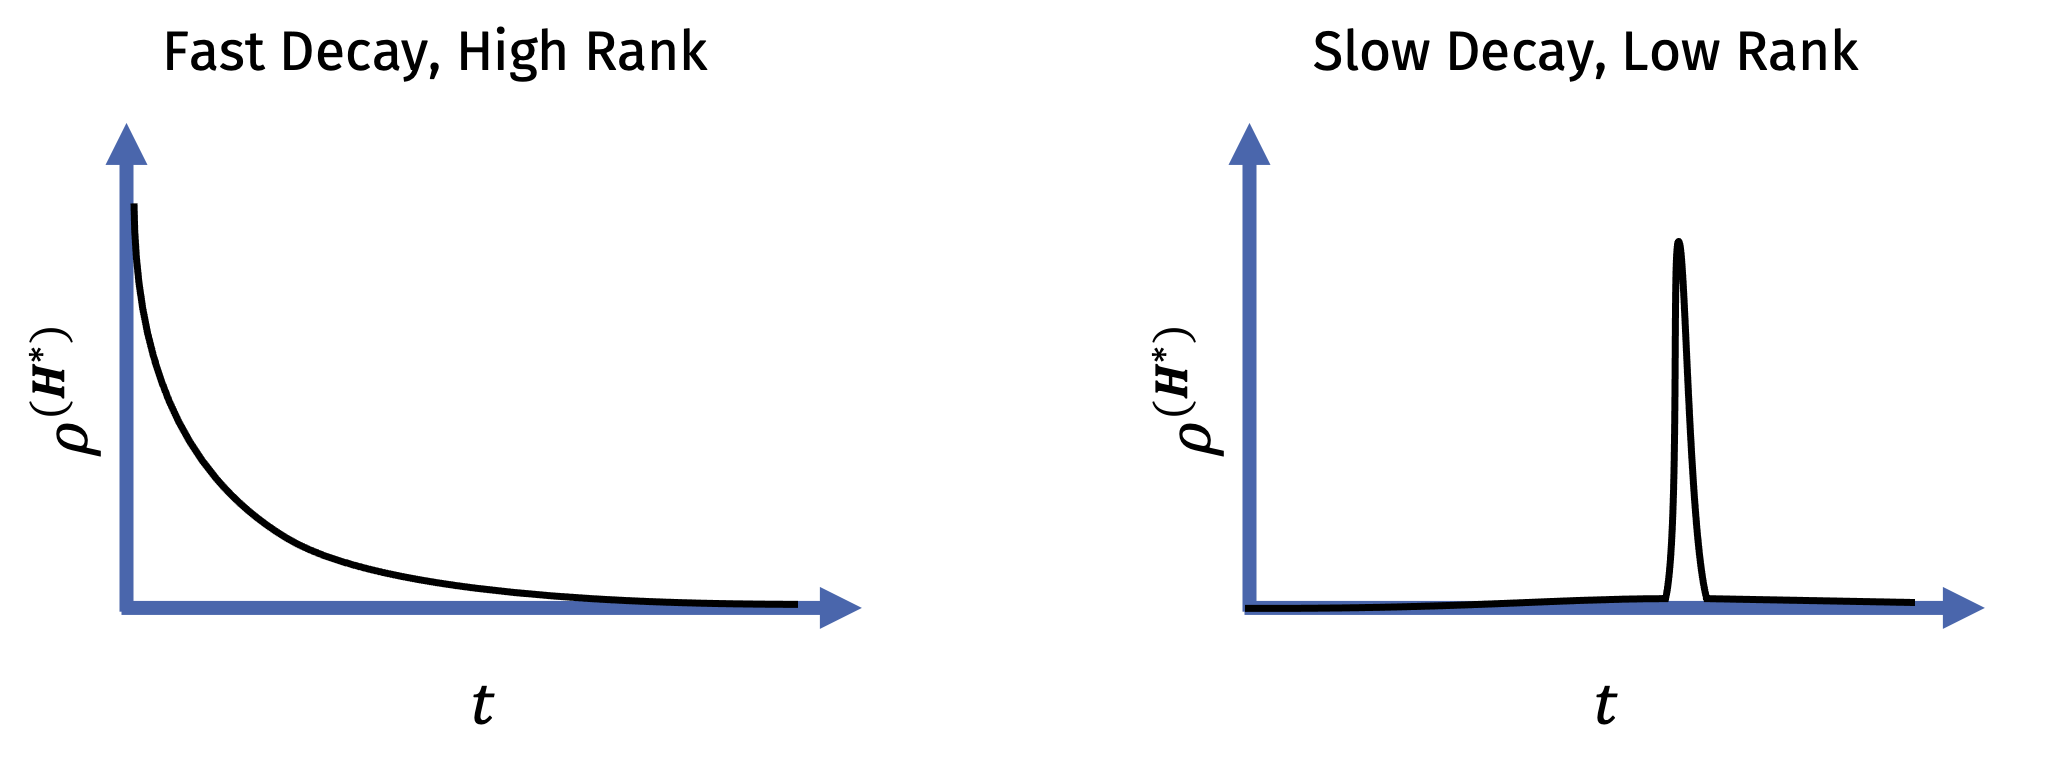
\includegraphics[width=0.9\textwidth]{figures/rnn_vs_cnn.png}
	\end{center}

\end{frame}
